\documentclass[aspectratio=169,12pt]{beamer}
\usepackage[utf8]{inputenc}
\usepackage{graphicx}
\usepackage{tikz}
\usepackage{listings}
\usepackage{hyperref}
\usepackage{booktabs}
\usepackage{multicol}
\usepackage{xcolor}
\usepackage{verbatim}
\usepackage{fontawesome5}

% Define JavaScript language for listings
\lstdefinelanguage{JavaScript}{
  keywords={typeof, new, true, false, catch, function, return, null, catch, switch, var, if, in, while, do, else, case, break, let, const, class, extends, super, import, export, from, default, async, await},
  keywordstyle=\color{blue}\bfseries,
  ndkeywords={constructor, prototype, this, Promise},
  ndkeywordstyle=\color{darkgray}\bfseries,
  identifierstyle=\color{black},
  sensitive=false,
  comment=[l]{//},
  morecomment=[s]{/*}{*/},
  commentstyle=\color{purple}\ttfamily,
  stringstyle=\color{red}\ttfamily,
  morestring=[b]',
  morestring=[b]"
}
% Define YAML language for listings
\lstdefinelanguage{yaml}{
  keywords={true,false,null,yes,no,on,off},
  keywordstyle=\color{darkgray}\bfseries,
  basicstyle=\ttfamily\footnotesize,
  sensitive=false,
  comment=[l]{\#},
  morecomment=[s]{/*}{*/},
  commentstyle=\color{purple}\ttfamily,
  stringstyle=\color{red}\ttfamily,
  morestring=[b]',
  morestring=[b]"
}

% Tambahkan definisi ini di preamble Anda

% Define HTML language for listings
\lstdefinelanguage{HTML5}{
  language=HTML,
  sensitive=true,
  alsoletter={-},
  morekeywords={application,command,dialog,dropdown,template,import,export,from,as,let,var,const,if,else,for,of,in,is,not,or,and,async,await,extends,implements,override,abstract,final,private,protected,public,readonly,static,get,set,constructor,super,this,new,delete,typeof,instanceof,void,true,false,null,undefined,symbol,bigint},
  morecomment=[s]{<!--}{-->},
  morecomment=[s]{/*}{*/},
  morestring=[b]',
  morestring=[b]",
  ndkeywords={id,class,href,src,alt,title,type,value,name,placeholder,action,method,enctype,accept-charset,target,rel,media,style,charset,lang,dir,translate,hidden,tabindex,accesskey,draggable,dropzone,contenteditable,contextmenu,spellcheck,data-,aria-,role},
  ndkeywordstyle=\color{blue}\bfseries,
  tagstyle=\color{magenta}\bfseries,
}

% Define SQL language for listings
\lstdefinelanguage{SQL}{
  morekeywords={ADD,ALTER,AND,AS,BEGIN,BETWEEN,BY,CASE,CREATE,COMMIT,CONSTRAINT,CONTINUE,CREATE,DATABASE,DECLARE,DEFAULT,DELETE,DROP,ELSE,END,ESCAPE,EXISTS,EXEC,EXECUTE,FETCH,FOR,FROM,GROUP,HAVING,IN,INDEX,INNER,INSERT,INTERSECT,INTO,IS,JOIN,KEY,LEFT,LIKE,NOT,NULL,ON,OR,ORDER,OUTER,PRIMARY,PROCEDURE,RELEASE,REPLACE,RETURN,ROLLBACK,SELECT,SET,TABLE,THEN,TO,TRANSACTION,UNION,UNIQUE,UPDATE,VALUES,WHERE,WHILE,WITH},
  sensitive=false,
  morecomment=[l]{--},
  morecomment=[s]{/*}{*/},
  morestring=[b]',
  morestring=[b]",
  keywordstyle=\color{blue}\bfseries,
  commentstyle=\color{purple}\ttfamily,
  stringstyle=\color{red}\ttfamily,
}

% Define Bash language for listings
\lstdefinelanguage{bash}{
  keywords={for,do,done,case,esac,if,then,elif,else,fi,while,until,function,select,echo,cd,ls,pwd,mkdir,rm,cp,mv,cat,grep,awk,sed,sudo,su,exit,return,export,local,read,source,alias,unalias,which,whereis,man,info,help,apt,yum,dnf,pacman,git,ssh,scp,rsync,curl,wget,ping,netstat,ps,top,kill,killall,nohup,bg,fg,jobs,history,tar,gzip,gunzip,zip,unzip,chmod,chown,chgrp,mount,umount,df,du,free,uname,uptime,whoami,who,w,id,date,cal,wc},
  keywordstyle=\color{blue}\bfseries,
  ndkeywords={true,false,yes,no},
  ndkeywordstyle=\color{darkgray}\bfseries,
  sensitive=false,
  comment=[l]{\#},
  morecomment=[s]{/*}{*/},
  commentstyle=\color{purple}\ttfamily,
  stringstyle=\color{red}\ttfamily,
  morestring=[b]',
  morestring=[b]"
}

% Set some basic styles for all listings
% You can also add some general settings for all listings
\lstset{
   basicstyle=\ttfamily\footnotesize,
   breaklines=true,
   frame=single,
   numbers=left,
   numberstyle=\tiny\color{gray},
   showstringspaces=false % Don't show spaces in strings
}



\usetheme{Madrid}
\usecolortheme{whale}
\setbeamertemplate{navigation symbols}{}

\definecolor{codegreen}{rgb}{0,0.6,0}
\definecolor{codegray}{rgb}{0.5,0.5,0.5}
\definecolor{codepurple}{rgb}{0.58,0,0.82}
\definecolor{backcolour}{rgb}{0.95,0.95,0.92}
\definecolor{alertred}{rgb}{0.8,0.1,0.1}
\definecolor{alertgreen}{rgb}{0.1,0.8,0.1}

\lstdefinestyle{mystyle}{
    backgroundcolor=\color{backcolour},   
    commentstyle=\color{codegreen},
    keywordstyle=\color{magenta},
    numberstyle=\tiny\color{codegray},
    stringstyle=\color{codepurple},
    basicstyle=\ttfamily\footnotesize,
    breakatwhitespace=false,         
    breaklines=true,                 
    captionpos=b,                    
    keepspaces=true,                 
    numbers=left,                    
    numbersep=5pt,                  
    showspaces=false,                
    showstringspaces=false,
    showtabs=false,                  
    tabsize=2
}
\lstset{style=mystyle}

\title{Day 1: Web Application Architecture and Fundamentals}
\subtitle{Comprehensive Training with Practical Examples and Hands-on Exercises}
\author{Security Training Team}
\institute{Web Application Security Department}
\date{\today}

\begin{document}

\begin{frame}
\titlepage
\end{frame}

\begin{frame}{Training Objectives}
\begin{columns}
\column{0.5\textwidth}
\textbf{Learning Outcomes:}
\begin{itemize}
\item[\faIcon{check-circle}] Understand web application architecture components
\item[\faIcon{check-circle}] Identify security implications of different architectures
\item[\faIcon{check-circle}] Analyze component interactions and data flow
\item[\faIcon{check-circle}] Apply security architecture principles
\end{itemize}
\column{0.5\textwidth}
\textbf{Practical Skills:}
\begin{itemize}
\item[\faIcon{laptop-code}] Architecture analysis techniques
\item[\faIcon{tools}] Security assessment methodologies
\item[\faIcon{shield-alt}] Security implementation strategies
\item[\faIcon{clipboard-check}]{Hands-on lab exercises}
\end{itemize}
\end{columns}
\end{frame}

\begin{frame}{Web Application Architecture Overview}
\begin{columns}
\column{0.6\textwidth}
\textbf{Core Architecture Components:}
\begin{enumerate}
\item \textbf{Client-Side Layer}
\begin{itemize}
\item Web browsers and mobile clients
\item Frontend frameworks and libraries
\item User interface components
\end{itemize}
\item \textbf{Server-Side Layer}
\begin{itemize}
\item Web servers (Apache, Nginx, IIS)
\item Application servers (Tomcat, WildFly)
\item API gateways and load balancers
\end{itemize}
\item \textbf{Data Layer}
\begin{itemize}
\item Databases (SQL, NoSQL)
\item Caching systems (Redis, Memcached)
\item File storage and object storage
\end{itemize}
\item \textbf{Infrastructure Layer}
\begin{itemize}
\item Network components and firewalls
\item Cloud services and containers
\item Monitoring and logging systems
\end{itemize}
\end{enumerate}
\column{0.4\textwidth}
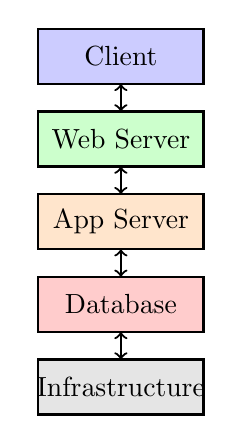
\begin{tikzpicture}[scale=0.7]
\draw[thick, fill=blue!20] (0,4) rectangle (3,5) node[pos=.5] {Client};
\draw[thick, fill=green!20] (0,2.5) rectangle (3,3.5) node[pos=.5] {Web Server};
\draw[thick, fill=orange!20] (0,1) rectangle (3,2) node[pos=.5] {App Server};
\draw[thick, fill=red!20] (0,-0.5) rectangle (3,0.5) node[pos=.5] {Database};
\draw[thick, fill=gray!20] (0,-2) rectangle (3,-1) node[pos=.5] {Infrastructure};
\draw[<->,thick] (1.5,4) -- (1.5,3.5);
\draw[<->,thick] (1.5,2.5) -- (1.5,2);
\draw[<->,thick] (1.5,1) -- (1.5,0.5);
\draw[<->,thick] (1.5,-0.5) -- (1.5,-1);
\end{tikzpicture}
\end{columns}
\end{frame}

\begin{frame}{Architecture Patterns and Security Implications}
\begin{columns}
\column{0.5\textwidth}
\textbf{Common Architecture Patterns:}
\begin{enumerate}
\item \textbf{Monolithic Architecture}
\begin{itemize}
\item Single deployable unit
\item Tight coupling between components
\item Security: Single point of failure
\end{itemize}
\item \textbf{Microservices Architecture}
\begin{itemize}
\item Distributed services
\item Loose coupling
\item Security: Multiple attack surfaces
\end{itemize}
\item \textbf{Serverless Architecture}
\begin{itemize}
\item Event-driven functions
\item No server management
\item Security: Third-party dependencies
\end{itemize}
\item \textbf{Progressive Web Apps}
\begin{itemize}
\item Mobile-like web experiences
\item Offline capabilities
\item Security: Service worker security
\end{itemize}
\end{enumerate}
\column{0.5\textwidth}
\textbf{Security Considerations by Pattern:}
\begin{table}
\centering
\small
\begin{tabular}{ll}
\toprule
\textbf{Pattern} & \textbf{Security Focus} \\
\midrule
Monolithic & Code security, patching \\
Microservices & API security, auth \\
Serverless & Function security, IAM \\
PWA & CSP, service workers \\
\bottomrule
\end{tabular}
\end{table}
\vspace{0.5cm}
\textbf{Security Architecture Principles:}
\begin{itemize}
\item[\faIcon{shield-alt}] Defense in Depth
\item[\faIcon{key}] Least Privilege
\item[\faIcon{lock}] Fail Secure
\item[\faIcon{eye}] Zero Trust
\end{itemize}
\end{columns}
\end{frame}

\begin{frame}[fragile]{Client-Side Components: Technologies and Security}
\begin{columns}
\column{0.5\textwidth}
\textbf{Frontend Technologies:}
\begin{itemize}
\item \textbf{HTML5} - Structure and semantics
\item \textbf{CSS3} - Styling and animations
\item \textbf{JavaScript} - Interactivity and logic
\item \textbf{Frameworks:}
\begin{itemize}
\item React - Component-based UI
\item Angular - Full-featured framework
\item Vue.js - Progressive framework
\item Svelte - Compile-time framework
\end{itemize}
\end{itemize}
\textbf{Security Vulnerabilities:}
\begin{itemize}
\item[\faIcon{exclamation-triangle}] Cross-Site Scripting (XSS)
\item[\faIcon{exclamation-triangle}] Cross-Site Request Forgery (CSRF)
\item[\faIcon{exclamation-triangle}]{Content Security Policy violations}
\item[\faIcon{exclamation-triangle}]{Insecure third-party libraries}
\end{itemize}
\column{0.5\textwidth}
\textbf{Secure HTML Example:}
\begin{lstlisting}[language=HTML]
<!DOCTYPE html>
<html lang="en">
<head>
    <meta charset="UTF-8">
    <meta http-equiv="X-UA-Compatible" 
          content="IE=edge">
    <meta name="viewport" 
          content="width=device-width, 
                   initial-scale=1.0">
    <!-- Security Headers -->
    <meta http-equiv="Content-Security-Policy" 
          content="default-src 'self'; 
                   script-src 'self' 'unsafe-inline';
                   style-src 'self' 'unsafe-inline'">
    <meta http-equiv="X-Content-Type-Options" 
          content="nosniff">
    <meta http-equiv="X-Frame-Options" 
          content="DENY">
</head>
<body>
    <!-- Secure form with CSRF protection -->
    <form action="/submit" method="POST">
        <input type="hidden" 
               name="csrf_token" 
               value="{{csrf_token}}">
        <!-- Input validation -->
        <input type="email" 
               name="email" 
               required 
               pattern="[a-z0-9._%+-]+@[a-z0-9.-]+\.[a-z]{2,}$">
        <button type="submit">Submit</button>
    </form>
</body>
</html>
\end{lstlisting}
\end{columns}
\end{frame}

\begin{frame}[fragile]{Server-Side Components: Technologies and Security}
\begin{columns}
\column{0.5\textwidth}
\textbf{Backend Technologies:}
\begin{itemize}
\item \textbf{PHP} - Server-side scripting
\begin{itemize}
\item Laravel, Symfony frameworks
\item WordPress, Drupal CMS
\end{itemize}
\item \textbf{ASP.NET} - Microsoft ecosystem
\begin{itemize}
\item ASP.NET Core, MVC
\item Entity Framework ORM
\end{itemize}
\item \textbf{Node.js} - JavaScript runtime
\begin{itemize}
\item Express, Nest.js frameworks
\item Real-time applications
\end{itemize}
\item \textbf{Python} - Django, Flask
\item \textbf{Java} - Spring Boot, JSP
\item \textbf{Ruby} - Ruby on Rails
\end{itemize}
\column{0.5\textwidth}
\textbf{Secure Node.js Example:}
\begin{lstlisting}[language=JavaScript]
const express = require('express');
const helmet = require('helmet');
const rateLimit = require('express-rate-limit');
const { body, validationResult } = require('express-validator');

const app = express();

// Security middleware
app.use(helmet());
app.use(express.json({ limit: '10kb' }));

// Rate limiting
const limiter = rateLimit({
    windowMs: 15 * 60 * 1000, // 15 minutes
    max: 100 // limit each IP to 100 requests per windowMs
});
app.use('/api/', limiter);

// Input validation
app.post('/api/user', [
    body('email').isEmail().normalizeEmail(),
    body('password').isLength({ min: 8 })
], (req, res) => {
    const errors = validationResult(req);
    if (!errors.isEmpty()) {
        return res.status(400).json({ errors: errors.array() });
    }
    
    // Process validated input
    const { email, password } = req.body;
    // Secure password hashing
    const hashedPassword = bcrypt.hashSync(password, 10);
    
    res.json({ message: 'User created successfully' });
});

// Error handling
app.use((err, req, res, next) => {
    console.error(err.stack);
    res.status(500).json({ error: 'Something went wrong!' });
});
\end{lstlisting}
\end{columns}
\end{frame}

\begin{frame}[fragile]{Database Layer: Types and Security}
\begin{columns}
\column{0.5\textwidth}
\textbf{Database Types:}
\begin{itemize}
\item \textbf{SQL Databases:}
\begin{itemize}
\item MySQL - Open source relational
\item PostgreSQL - Advanced features
\item SQL Server - Microsoft ecosystem
\item Oracle - Enterprise solutions
\end{itemize}
\item \textbf{NoSQL Databases:}
\begin{itemize}
\item MongoDB - Document-based
\item Redis - In-memory caching
\item Cassandra - Distributed
\item Elasticsearch - Search engine
\end{itemize}
\item \textbf{Object Storage:}
\begin{itemize}
\item Amazon S3
\item Google Cloud Storage
\item Azure Blob Storage
\end{itemize}
\end{itemize}
\textbf{Database Security Best Practices:}
\begin{itemize}
\item[\faIcon{shield-alt}] Principle of least privilege
\item[\faIcon{lock}] Encryption at rest and in transit
\item[\faIcon{user-shield}] Regular security audits
\item[\faIcon{database}] Backup and recovery planning
\end{itemize}
\column{0.5\textwidth}
\textbf{Secure Database Configuration:}
\begin{lstlisting}[language=SQL]
-- MySQL Security Configuration
CREATE USER 'secure_user'@'localhost' 
IDENTIFIED BY 'StrongPassword123!';

-- Grant minimal required privileges
GRANT SELECT, INSERT, UPDATE, DELETE 
ON webapp_database.* 
TO 'secure_user'@'localhost';

-- Remove unnecessary privileges
REVOKE ALL PRIVILEGES, GRANT OPTION 
FROM 'old_user'@'%';

-- Enable SSL connections
[mysqld]
ssl-ca=/path/to/ca.pem
ssl-cert=/path/to/server-cert.pem
ssl-key=/path/to/server-key.pem

-- Set secure parameters
[mysqld]
bind-address = 127.0.0.1
max_connections = 100
skip-networking = 0
\end{lstlisting}
\end{columns}
\end{frame}

\begin{frame}[fragile]{Component Interactions and Communication Security}
\begin{columns}
\column{0.6\textwidth}
\textbf{Communication Protocols:}
\begin{itemize}
\item \textbf{HTTP/HTTPS}
\begin{itemize}
\item RESTful APIs
\item SOAP web services
\item GraphQL APIs
\end{itemize}
\item \textbf{Real-time Communication}
\begin{itemize}
\item WebSockets
\item Server-Sent Events
\item WebRTC
\end{itemize}
\item \textbf{Message Queues}
\begin{itemize}
\item RabbitMQ
\item Apache Kafka
\item Redis Pub/Sub
\end{itemize}
\end{itemize}
\textbf{Security Considerations:}
\begin{itemize}
\item[\faIcon{lock}] Always use HTTPS/TLS
\item[\faIcon{certificate}] Implement certificate pinning
\item[\faIcon{ban}] Disable insecure protocols
\item[\faIcon{user-secret}]{Authentication and authorization}
\end{itemize}
\column{0.4\textwidth}
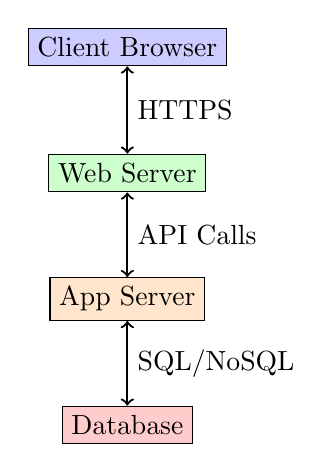
\begin{tikzpicture}[scale=0.8]
\node[draw, rectangle, fill=blue!20] (client) at (0,3) {Client Browser};
\node[draw, rectangle, fill=green!20] (web) at (0,1) {Web Server};
\node[draw, rectangle, fill=orange!20] (app) at (0,-1) {App Server};
\node[draw, rectangle, fill=red!20] (db) at (0,-3) {Database};

\draw[<->, thick] (client) -- (web) node[midway, right] {HTTPS};
\draw[<->, thick] (web) -- (app) node[midway, right] {API Calls};
\draw[<->, thick] (app) -- (db) node[midway, right] {SQL/NoSQL};
\end{tikzpicture}
\vspace{0.5cm}
\textbf{Security Headers:}
\begin{itemize}
\item[\faIcon{shield-alt}] HSTS
\item[\faIcon{shield-alt}] CSP
\item[\faIcon{shield-alt}] X-Frame-Options
\item[\faIcon{shield-alt}]{X-Content-Type-Options}
\end{itemize}
\end{columns}
\end{frame}

\begin{frame}[fragile]{Security Architecture Principles in Practice}
\begin{columns}
\column{0.5\textwidth}
\textbf{Defense in Depth Implementation:}
\begin{enumerate}
\item \textbf{Network Layer}
\begin{itemize}
\item Firewalls and WAFs
\item IDS/IPS systems
\item Network segmentation
\end{itemize}
\item \textbf{Host Layer}
\begin{itemize}
\item Operating system hardening
\item Antivirus/EDR solutions
\item File integrity monitoring
\end{itemize}
\item \textbf{Application Layer}
\begin{itemize}
\item Input validation
\item Output encoding
\item Access controls
\end{itemize}
\item \textbf{Data Layer}
\begin{itemize}
\item Encryption at rest
\item Data masking
\item Access logging
\end{itemize}
\end{enumerate}
\column{0.5\textwidth}
\textbf{Secure Configuration Example:}
\begin{lstlisting}[language=bash]
# Nginx Security Configuration
server {
    listen 443 ssl http2;
    server_name example.com;
    
    # SSL/TLS Configuration
    ssl_certificate /etc/ssl/certs/cert.pem;
    ssl_certificate_key /etc/ssl/private/key.pem;
    ssl_protocols TLSv1.2 TLSv1.3;
    ssl_ciphers HIGH:!aNULL:!MD5;
    
    # Security Headers
    add_header X-Frame-Options "SAMEORIGIN" always;
    add_header X-Content-Type-Options "nosniff" always;
    add_header X-XSS-Protection "1; mode=block" always;
    add_header Strict-Transport-Security "max-age=31536000; includeSubDomains" always;
    
    # Rate Limiting
    limit_req_zone $binary_remote_addr zone=api:10m rate=10r/s;
    limit_req zone=api burst=20 nodelay;
    
    # File Access Control
    location / {
        root /var/www/html;
        index index.html;
        try_files $uri $uri/ =404;
    }
    
    # Block access to sensitive files
    location ~* \.(env|log|conf)$ {
        deny all;
    }
}
\end{lstlisting}
\end{columns}
\end{frame}

\begin{frame}{Hands-on Lab: Architecture Analysis and Security Assessment}
\begin{columns}
\column{0.5\textwidth}
\textbf{Lab Objectives:}
\begin{itemize}
\item[\faIcon{bullseye}] Identify components in a web application
\item[\faIcon{map}] Map data flow between components
\item[\faIcon{search}] Identify potential security vulnerabilities
\item[\faIcon{shield-alt}] Recommend security improvements
\end{itemize}
\textbf{Lab Environment Setup:}
\begin{enumerate}
\item Install Docker and Docker Compose
\item Clone vulnerable web application repository
\item Set up security scanning tools
\item Configure logging and monitoring
\end{enumerate}
\textbf{Tools Required:}
\begin{itemize}
\item[\faIcon{tools}] Nmap for network scanning
\item[\faIcon{tools}] OWASP ZAP for web app scanning
\item[\faIcon{tools}] Burp Suite for proxy testing
\item[\faIcon{tools}]{Nikto for server scanning}
\end{itemize}
\column{0.5\textwidth}
\textbf{Lab Tasks:}
\begin{enumerate}
\item \textbf{Architecture Analysis}
\begin{itemize}
\item Document all application components
\item Identify technology stack
\item Map data flow diagrams
\item Identify entry points and exit points
\end{itemize}
\item \textbf{Security Assessment}
\begin{itemize}
\item Perform vulnerability scanning
\item Identify misconfigurations
\item Check for insecure dependencies
\item Analyze authentication mechanisms
\end{itemize}
\item \textbf{Security Implementation}
\begin{itemize}
\item Implement security headers
\item Configure input validation
\item Set up access controls
\item Create monitoring alerts
\end{itemize}
\item \textbf{Documentation}
\begin{itemize}
\item Create architecture diagrams
\item Document security findings
\item Create remediation plan
\item Develop security policies
\end{itemize}
\end{enumerate}
\end{columns}
\end{frame}

% Frame removed due to compilation issues

\begin{frame}{Security Assessment Checklist}
\begin{columns}
\column{0.5\textwidth}
\textbf{Architecture Security Checklist:}
\begin{enumerate}
\item \textbf{Network Security}
\begin{itemize}
\item[\faIcon{check}] Firewall rules configured
\item[\faIcon{check}] Network segmentation implemented
\item[\faIcon{check}] Intrusion detection enabled
\item[\faIcon{check}]{DDoS protection in place}
\end{itemize}
\item \textbf{Host Security}
\begin{itemize}
\item[\faIcon{check}] OS hardening applied
\item[\faIcon{check}] Regular updates maintained
\item[\faIcon{check}] File permissions secured
\item[\faIcon{check}]{Antivirus/EDR deployed}
\end{itemize}
\item \textbf{Application Security}
\begin{itemize}
\item[\faIcon{check}] Input validation implemented
\item[\faIcon{check}] Output encoding applied
\item[\faIcon{check}] Authentication secured
\item[\faIcon{check}]{Authorization enforced}
\end{itemize}
\column{0.5\textwidth}
\textbf{Data Security Checklist:}
\begin{enumerate}
\item \textbf{Encryption}
\begin{itemize}
\item[\faIcon{check}] Data at rest encrypted
\item[\faIcon{check}] Data in transit encrypted
\item[\faIcon{check}] Key management secured
\item[\faIcon{check}]{Backup encryption enabled}
\end{itemize}
\item \textbf{Access Control}
\begin{itemize}
\item[\faIcon{check}] Principle of least privilege
\item[\faIcon{check}] Role-based access control
\item[\faIcon{check}] Multi-factor authentication
\item[\faIcon{check}]{Regular access reviews}
\end{itemize}
\item \textbf{Monitoring}
\begin{itemize}
\item[\faIcon{check}] Logging implemented
\item[\faIcon{check}] Alerting configured
\item[\faIcon{check}] Auditing enabled
\item[\faIcon{check}]{Security testing scheduled}
\end{itemize}
\end{enumerate}
\end{columns}
\end{frame}

\begin{frame}{Summary and Key Takeaways}
\begin{columns}
\column{0.5\textwidth}
\textbf{Architecture Fundamentals:}
\begin{itemize}
\item[\faIcon{building}] Understanding web app layers
\item[\faIcon{network-wired}] Component interactions
\item[\faIcon{sitemap}] Data flow mapping
\item[\faIcon{cogs}] Technology selection impact
\end{itemize}
\textbf{Security Considerations:}
\begin{itemize}
\item[\faIcon{shield-alt}] Defense in depth
\item[\faIcon{key}] Least privilege principle
\item[\faIcon{lock}] Fail secure approach
\item[\faIcon{eye}] Zero trust architecture
\end{itemize}
\column{0.5\textwidth}
\textbf{Practical Implementation:}
\begin{itemize}
\item[\faIcon{code}] Secure coding practices
\item[\faIcon{tools}]{Security tool integration}
\item[\faIcon{clipboard-check}]{Regular security assessments}
\item[\faIcon{book}]{Documentation and policies}
\end{itemize}
\textbf{Next Steps:}
\begin{itemize}
\item[\faIcon{arrow-right}] Apply concepts to real projects
\item[\faIcon{arrow-right}] Conduct security audits
\item[\faIcon{arrow-right}] Implement security controls
\item[\faIcon{arrow-right}]{Continuous improvement}
\end{itemize}
\end{columns}
\vspace{0.5cm}
\begin{center}
\Large{\textbf{Questions?}}\\
\vspace{0.3cm}
\normalsize{Contact: security-team@organization.com}\\
\vspace{0.2cm}
\small{Additional Resources: OWASP Foundation, NIST Cybersecurity Framework}
\end{center}
\end{frame}

\end{document}
